%!Mode:: "TeX:UTF-8"
\documentclass[a4paper,11pt,UTF8]{ctexart}

\usepackage{indentfirst} %缩进
\usepackage{xeCJK}    %使用系统字体
\usepackage{fancyhdr} %自定义页眉页脚
\pagestyle{empty}                   %不设置页眉页脚
\usepackage{amsmath, amsthm, amssymb, amsfonts} %数学公式
\usepackage[a4paper,left=3cm,right=3cm,top=3cm,bottom=3cm]{geometry}
%\usepackage[tmargin=1in,bmargin=1in,lmargin=1.25in,rmargin=1.25in]{geometry}.
\usepackage{booktabs} %插入表格
\usepackage[section]{placeins} %避免浮动
\usepackage{listings} %插入代码
\usepackage{ctex}     %中文宏包
\usepackage[svgnames, table]{xcolor} %彩色表格
\usepackage{algorithm}          %伪代码
\usepackage{algorithmicx}
\usepackage{algpseudocode}
\usepackage{algorithm,algpseudocode,float}
\usepackage{lipsum}
\usepackage{enumitem}           %调整列举环境
\usepackage{url}
\usepackage{fontspec,xunicode}
\defaultfontfeatures{Mapping=tex-text} %如果没有它,会有一些 tex 特殊字符无法正常使用,比如连字符。

\usepackage{graphicx}
\graphicspath{{imgs/}}

%%%%%%%%%%%%%%%%%%%%%%%%%%%%%%%%%%%%%%%%%%%%%%%%%%%%%%%%%%%%%%%%
% 缩进及行间距
%%%%%%%%%%%%%%%%%%%%%%%%%%%%%%%%%%%%%%%%%%%%%%%%%%%%%%%%%%%%%%%%
\setlength{\parindent}{22pt} %重新定义缩进长度
\setlength{\baselineskip}{20pt}  %定义行间距
%\renewcommand{\baselinestretch}{1.1} %定义行间距

%%%%%%%%%%%%%%%%%%%%%%%%%%%%%%%%%%%%%%%%%%%%%%%%%%%%%%%%%%%%%%%%
% 列表设置
%%%%%%%%%%%%%%%%%%%%%%%%%%%%%%%%%%%%%%%%%%%%%%%%%%%%%%%%%%%%%%%%
\setenumerate{fullwidth,itemindent=\parindent,listparindent=\parindent,itemsep=0ex,partopsep=0pt,parsep=0ex}
\setenumerate[2]{label=\alph*),leftmargin=1.5em}  %二级item设置
\setitemize{itemindent=38pt,leftmargin=0pt,itemsep=-0.4ex,listparindent=26pt,partopsep=0pt,parsep=0.5ex,topsep=-0.25ex}
\setdescription{itemindent=38pt,leftmargin=0pt,itemsep=-0.4ex,listparindent=26pt,partopsep=0pt,parsep=0.5ex,topsep=-0.25ex}

%%%%%%%%%%%%%%%%%%%%%%%%%%%%%%%%%%%%%%%%%%%%%%%%%%%%%%%%%%%%%%%%
% 图的标题行间距设置
%%%%%%%%%%%%%%%%%%%%%%%%%%%%%%%%%%%%%%%%%%%%%%%%%%%%%%%%%%%%%%%%
\newcommand{\bottomcaption}{%
\setlength{\abovecaptionskip}{6pt}%
\setlength{\belowcaptionskip}{6pt}%
\caption}


%%%%%%%%%%%%%%%%%%%%%%%%%%%%%%%%%%%%%%%%%%%%%%%%%%%%%%%%%%%%%%%%
% 字体定义
%%%%%%%%%%%%%%%%%%%%%%%%%%%%%%%%%%%%%%%%%%%%%%%%%%%%%%%%%%%%%%%%
\setmainfont{Times New Roman}  %默认英文字体.serif是有衬线字体sans serif无衬线字体
\setmonofont{Consolas}
\setCJKmainfont[ItalicFont={楷体}, BoldFont={黑体}]{宋体}%衬线字体 缺省中文字体为
\setCJKsansfont{黑体}
\punctstyle{hangmobanjiao}
%-----------------------xeCJK下设置中文字体------------------------------%
\setCJKfamilyfont{song}{SimSun}                             %宋体 song
\newcommand{\song}{\CJKfamily{song}}
\setCJKfamilyfont{fs}{FangSong}                      %仿宋  fs
\newcommand{\fs}{\CJKfamily{fs}}
\setCJKfamilyfont{ktgb}{KaiTi}                      %楷体2312 ktgb
\newcommand{\ktgb}{\CJKfamily{ktgb}}
\setCJKfamilyfont{yh}{Microsoft YaHei}                    %微软雅黑 yh
\newcommand{\yh}{\CJKfamily{yh}}
\setCJKfamilyfont{hei}{SimHei}                              %黑体  hei
\newcommand{\hei}{\CJKfamily{hei}}
\setCJKfamilyfont{hwxk}{STXingkai}                                %华文行楷  hwxk
\newcommand{\hwxk}{\CJKfamily{hwxk}}
%------------------------------设置字体大小------------------------%
\newcommand{\shiyanbaogao}{\fontsize{36pt}{\baselineskip}\selectfont}
\newcommand{\chuhao}{\fontsize{42pt}{\baselineskip}\selectfont}     %初号
\newcommand{\xiaochuhao}{\fontsize{36pt}{\baselineskip}\selectfont} %小初号
\newcommand{\yihao}{\fontsize{28pt}{\baselineskip}\selectfont}      %一号
\newcommand{\erhao}{\fontsize{21pt}{\baselineskip}\selectfont}      %二号
\newcommand{\xiaoerhao}{\fontsize{18pt}{\baselineskip}\selectfont}  %小二号
\newcommand{\sanhao}{\fontsize{15.75pt}{\baselineskip}\selectfont}  %三号
\newcommand{\sihao}{\fontsize{14pt}{\baselineskip}\selectfont}       %四号
\newcommand{\xiaosihao}{\fontsize{12pt}{\baselineskip}\selectfont}  %小四号
\newcommand{\wuhao}{\fontsize{10.5pt}{\baselineskip}\selectfont}    %五号
\newcommand{\xiaowuhao}{\fontsize{9pt}{\baselineskip}\selectfont}   %小五号
\newcommand{\liuhao}{\fontsize{7.875pt}{\baselineskip}\selectfont}  %六号
\newcommand{\qihao}{\fontsize{5.25pt}{\baselineskip}\selectfont}    %七号

%%%%%%%%%%%%%%%%%%%%%%%%%%%%%%%%%%%%%%%%%%%%%%%%%%%%%%%%%%%%%%%%
% 图题字体大小相同
%%%%%%%%%%%%%%%%%%%%%%%%%%%%%%%%%%%%%%%%%%%%%%%%%%%%%%%%%%%%%%%%
\usepackage{caption}
\captionsetup{font={footnotesize}}   % footnotesize = 9pt
\captionsetup[lstlisting]{font={footnotesize}}

%%%%%%%%%%%%%%%%%%%%%%%%%%%%%%%%%%%%%%%%%%%%%%%%%%%%%%%%%%%%%%%%
% 重定义枚举编号为 1),2)...
%%%%%%%%%%%%%%%%%%%%%%%%%%%%%%%%%%%%%%%%%%%%%%%%%%%%%%%%%%%%%%%%
\renewcommand{\labelenumi}{\theenumi)}

%%%%%%%%%%%%%%%%%%%%%%%%%%%%%%%%%%%%%%%%%%%%%%%%%%%%%%%%%%%%%%%%
% 标题名称中文化
%%%%%%%%%%%%%%%%%%%%%%%%%%%%%%%%%%%%%%%%%%%%%%%%%%%%%%%%%%%%%%%%
\renewcommand\figurename{\hei 图}
\renewcommand\tablename{\hei 表}
\renewcommand\lstlistingname{\hei 代码}
\renewcommand{\algorithmicrequire}{\textbf{输入:}}
\renewcommand{\algorithmicensure}{\textbf{输出:}}
\newtheorem{define}{定义}

%%%%%%%%%%%%%%%%%%%%%%%%%%%%%%%%%%%%%%%%%%%%%%%%%%%%%%%%%%%%%%%%
% 代码设置
%%%%%%%%%%%%%%%%%%%%%%%%%%%%%%%%%%%%%%%%%%%%%%%%%%%%%%%%%%%%%%%%
\lstset{
 columns=fixed,
 numbers=left,                                        % 在左侧显示行号
 numberstyle=\tiny\color{gray},                       % 设定行号格式
 frame=single,                                        % 单线背景边框
 breaklines=true,                                     % 设定LaTeX对过长的代码行进行自动换行
 keywordstyle=\color[RGB]{40,40,255},                 % 设定关键字颜色
 numberstyle=\footnotesize\color{darkgray},
 commentstyle=\it\color[RGB]{0,96,96},                % 设置代码注释的格式
 stringstyle=\rmfamily\slshape\color[RGB]{128,0,0},   % 设置字符串格式
 showstringspaces=false,                              % 不显示字符串中的空格
 language=java,                                        % 设置语言
 basicstyle=\linespread{1.0}\xiaowuhao\ttfamily,                      % 字体字号
 %lineskip=10pt,
 %baselinestretch=1,
}

%%%%%%%%%%%%%%%%%%%%%%%%%%%%%%%%%%%%%%%%%%%%%%%%%%%%%%%%%%%%%%%%
% 伪代码分页
%%%%%%%%%%%%%%%%%%%%%%%%%%%%%%%%%%%%%%%%%%%%%%%%%%%%%%%%%%%%%%%%
\makeatletter
\renewcommand{\ALG@name}{算法}
\newenvironment{breakablealgorithm}
  {% \begin{breakablealgorithm}
   \begin{center}
     \refstepcounter{algorithm}% New algorithm
     \hrule height.8pt depth0pt \kern2pt% \@fs@pre for \@fs@ruled
     \renewcommand{\caption}[2][\relax]{% Make a new \caption
       {\raggedright\textbf{\ALG@name~\thealgorithm} ##2\par}%
       \ifx\relax##1\relax % #1 is \relax
         \addcontentsline{loa}{algorithm}{\protect\numberline{\thealgorithm}##2}%
       \else % #1 is not \relax
         \addcontentsline{loa}{algorithm}{\protect\numberline{\thealgorithm}##1}%
       \fi
       \kern2pt\hrule\kern2pt
     }
  }{% \end{breakablealgorithm}
     \kern2pt\hrule\relax% \@fs@post for \@fs@ruled
   \end{center}
  }
\makeatother

% =============================================
% Part 1 Edit the info
% =============================================

\newcommand{\major}{物理学院}
\newcommand{\name}{黄阅迅,李秋阳}
\newcommand{\stuid}{PB18020631,PB18020567}
\newcommand{\group}{20}
\newcommand{\newdate}{\today}


\newcommand{\course}{电子线路实验(1)}
\newcommand{\newtitle}{数据选择器}

% =============================================
% Part 1 Main document
% =============================================
\begin{document}
\thispagestyle{empty}
\begin{figure}[h]
  \begin{minipage}{0.6\linewidth}
    \centerline{
\includegraphics[width=\linewidth]{logo.png}}
  \end{minipage}
  \hfill
  \begin{minipage}{.4\linewidth}
    \raggedleft
    \begin{tabular*}{.8\linewidth}{ll}
      学院: & \underline\major   \\
      姓名: & \underline\name    \\
      学号: & \underline\stuid   \\
      组号:  & \underline\group   \\
      日期: & \underline\newdate \\
    \end{tabular*}
  \end{minipage}
\end{figure}

\begin{table}[!htbp]
  \centering
  \begin{tabular*}{\linewidth}{llllll}
    课程名称:  \underline\course   \qquad\qquad 实验题目:  \underline\newtitle  
  \end{tabular*}
\end{table}

% =============================================
% Part 2 Main document
% =============================================

%
\newcommand{\p}{\par}
\newcommand{\np}{\par\noindent}
%
\newcommand{\expa}{用8选1数据选择器74LS151设计三输入多数表决电路}
\newcommand{\expb}{用两片74LS151实现逻辑函数: $Y=\sum m(6,7,8,11,13)$}
\newcommand{\expc}{试用8选1数据选择器74LS151产生逻辑函数:
$Y=AC'D+BC+BC'D'+A'B'CD$}
\newcommand{\expd}{用双4选1数据选择器74LS153实现一位全加器}
\newcommand{\chip}{数据选择器74LS151}

\newcommand{\CI}{C\negthinspace I}
\newcommand{\CO}{C\negthinspace O}
%

\section{实验目的}

请参看预习报告。

\section{实验原理}

请参看预习报告。

\section{实验内容、步骤与结果}
 \subsection{实验一:\expa}
  \p 设三输入为 $A_0,\ A_1,\ A_2$,多数表决通过的逻辑函数为:
  \[ Y=A_2A_1A_0+A_2A_1A_0'+A_2A_1'A_0+A_2'A_1A_0 \]
  \p 逻辑表达式由4个最小项组成,所以,在\chip 中,需要将 $D_7,\ D_6,\ D_5,\ D_3$ 输入接高,其余接低。然后 $A_2,\ A_1,\ A_0$ 分别对应芯片三位输入的从高到低位,于是可得电路连线图:
  \begin{figure}[H]
   \centering
   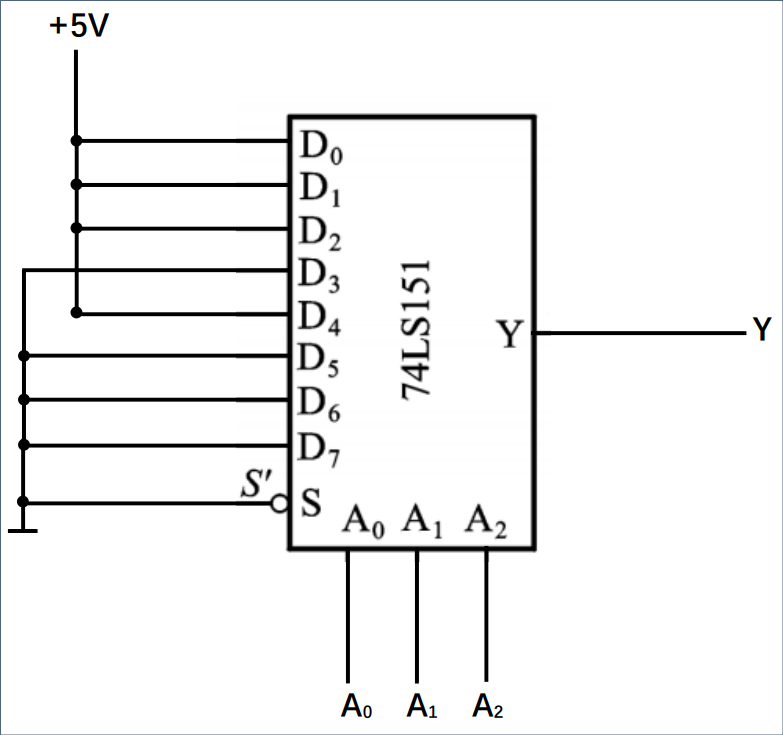
\includegraphics[width=6cm]{Exp01}
   \caption{实验一电路图}
   \label{fig:Exp01}
  \end{figure}
  \p 由此得到电路的真值表:
  \begin{table}[H]
   \centering
   \begin{tabular}{|ccc|c|}\hline
    \multicolumn{3}{|c|}{In} &Out
    \\\hline
    $A_2$ &$A_1$ &$A_0$ &$Y$
    \\\hline
    0 &0 &0 &0\\
    0 &0 &1 &0\\
    0 &1 &0 &0\\
    0 &1 &1 &1\\
    1 &0 &0 &0\\
    1 &0 &1 &1\\
    1 &1 &0 &1\\
    1 &1 &1 &1
    \\\hline
   \end{tabular}
   \caption{实验一真值表}
   \label{tab:Exp01}
  \end{table}
  
 \subsection{实验二:\expb}
  \p 因为最终结果是最小项之和,其中的最小项只要不是全为0,输出就为1。设 $A_3,\ A_2,\ A_1,\ A_0$ 分别为高到低位。
  \p 当 $A_3=0$ 时,任何 $m(k),\ k\geqslant 9$ 的最小项都一定为0,此时高位片不需要考虑,即给高片 $S'$ 输入0,不使能。
  \p 当 $A_3=0$ 时,任何 $m(k),\ k\leqslant 8$ 的最小项一定都为0,此时低位片不需要考虑,即给低片 $S'$ 输入0,不使能。
  \p 而某一片工作时,只需要给在结果中出现的最小项输入1,其余置0即可。于是得到电路图:
  \begin{figure}[H]
   \centering
   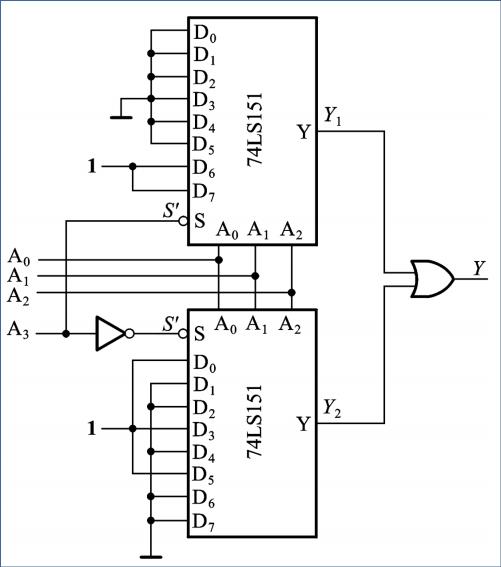
\includegraphics[width=6cm]{Exp02}
   \caption{实验二电路图}
   \label{fig:Exp02}
  \end{figure}
  \p 由此得到电路的真值表:
  \begin{table}[H]
   \centering
   \begin{tabular}{|cccc|c|cccc|c|}\hline
    \multicolumn{4}{|c|}{In} &Out 
    &\multicolumn{4}{|c|}{In} &Out
    \\\hline
    $A_3$ &$A_2$ &$A_1$ &$A_0$ &$Y$ &
    $A_3$ &$A_2$ &$A_1$ &$A_0$ &$Y$
    \\\hline
    0 &0 &0 &0	&0 &
    1 &0 &0 &0	&1\\
    0 &0 &0 &1	&0 &
    1 &0 &0 &1	&0\\
    0 &0 &1 &0	&0 &
    1 &0 &1 &0	&0\\
    0 &0 &1 &1	&0 &
    1 &0 &1 &1	&1\\
    0 &1 &0 &0	&0 &
    1 &1 &0 &0	&0\\
    0 &1 &0 &1	&0 &
    1 &1 &0 &1	&1\\
    0 &1 &1 &0	&1 &
    1 &1 &1 &0	&0\\
    0 &1 &1 &1	&1 &
    1 &1 &1 &1	&0
    \\\hline
   \end{tabular}
   \caption{实验二真值表}
   \label{tab:Exp02}
  \end{table}
  
 \subsection{实验三:\expc}
  \p 设 $A,\ ,B,\ C$ 为地址控制位,$D$ 为芯片接的输入信息。将逻辑函数化成最小项之和表达式:
  \begin{align*}
	 Y&=AC'D+BC+BC'D'+A'B'CD\\
	 &=ABC'D+AB'C'D+ABCD+A'BCD+ABCD'+A'BCD'\\
	 &\qquad+ABC'D'+A'BC'D'+A'B'CD\\
	 &=m_0\cdot0+m_1D+m_2D'+m_3\cdot1+m_4D
	 +m_5\cdot0+m_6\cdot1+m_7\cdot1
  \end{align*}
  \p 端口连接如下:
  \begin{center}
   \kaishu $D_0$ 接0,$D_1,\ D_4$ 接 $D$,$D_2$ 接 $D'$,$D_3,\ D_6,\ D_7$ 接1。
  \end{center}
  \p 由此得到电路连接图:
  \begin{figure}[H]
   \centering
   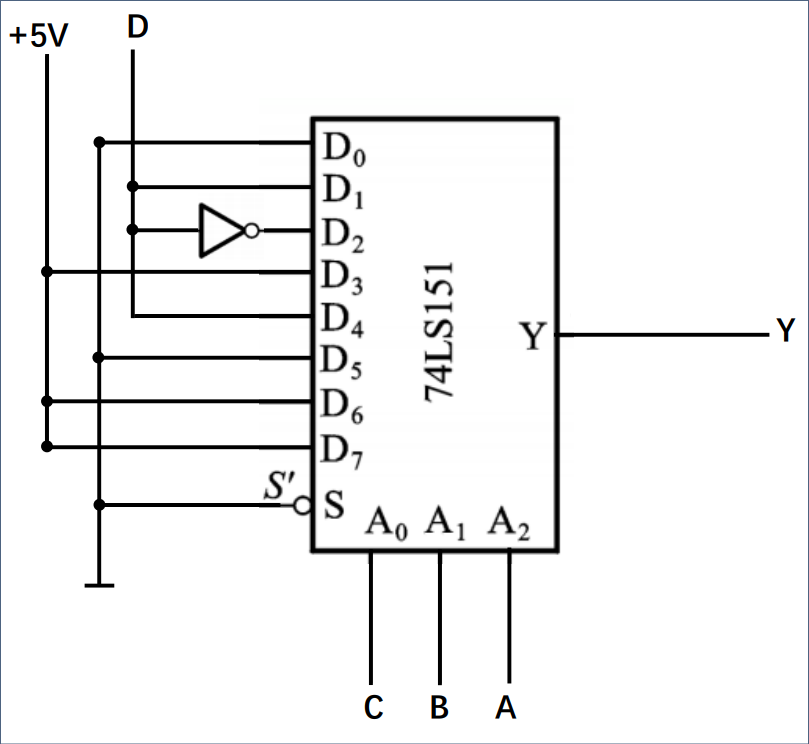
\includegraphics[width=6cm]{Exp03}
   \caption{实验三电路图}
   \label{fig:Exp03}
  \end{figure}
  \p 真值表如下:
  \begin{table}[H]
   \centering
   \begin{tabular}{|cccc|c|cccc|c|}\hline
    \multicolumn{4}{|c|}{In} &Out 
    &\multicolumn{4}{|c|}{In} &Out
    \\\hline
    $A$ &$B$ &$C$ &$D$ &$Y$ &
    $A_3$ &$A_2$ &$A_1$ &$A_0$ &$Y$
    \\\hline
    0 &0 &0 &0	&0 &
    1 &0 &0 &0	&0\\
    0 &0 &0 &1	&0 &
    1 &0 &0 &1	&1\\
    0 &0 &1 &0	&0 &
    1 &0 &1 &0	&0\\
    0 &0 &1 &1	&1 &
    1 &0 &1 &1	&0\\
    0 &1 &0 &0	&1 &
    1 &1 &0 &0	&1\\
    0 &1 &0 &1	&0 &
    1 &1 &0 &1	&1\\
    0 &1 &1 &0	&1 &
    1 &1 &1 &0	&1\\
    0 &1 &1 &1	&1 &
    1 &1 &1 &1	&1
    \\\hline
   \end{tabular}
   \caption{实验三真值表}
   \label{tab:Exp03}
  \end{table}

  
 \subsection{实验四:\expd}
  \p 在全加器中,$\CI$ 是输入的前一位进位标志,$A,\ B$ 为一位二进制待加数,$\CO$ 是输出的本位进位标志,$S$ 是本位的加法结果(计入前一位的进位)。其真值表为:
  \begin{table}[H]
   \centering
   \begin{tabular}{|ccc|cc|}\hline
    $A$ &$B$ &$\CI$ &$S$ &$\CO$
    \\\hline
    0 &0 &0		&0 &0\\
    0 &0 &1 	&1 &0\\
    0 &1 &0 	&1 &0\\
    0 &1 &1 	&0 &1\\
    1 &0 &0 	&1 &0\\
    1 &0 &1 	&0 &1\\
    1 &1 &0 	&0 &1\\
    1 &1 &1 	&1 &1
    \\\hline
   \end{tabular}
   \caption{实验四真值表}
   \label{tab:Exp04}
  \end{table}
  \p 由此可以得到输出量的逻辑表达式。设 $A\to A_1,\ B\to A_0$ 分别为高、低位选址信号,而 $\CI$ 作为输入在 $D$ 输入端口的信号,那么:
  \[ S=A'B'\CI+A'B\CI'+AB'CI'+AB\CI=m_0\CI+m_1\CI'+m_2\CI'
  +m_3\CI \]
  \[ \CO=A'B\CI+AB'\CI+AB=m_0\cdot0+m_1\CI+m_2\CI+m_3\cdot1 \]
  \p 若假设 $S$ 用2号数据选择器,$\CO$ 用1号数据选择器,那么端口连接如下:
  \begin{center}
   \kaishu $D_{20},\ D_{23}$ 连 $\CI$,$D_{21},\ D_{22}$ 连 $\CI'$;
  \p $D{1_0}$ 连0,$D_{11},\ D_{12}$ 连 $\CI$,$D_{13}$ 连1。
  \end{center}

  
  \p 由此得到电路连接图:
  \begin{figure}[H]
   \centering
   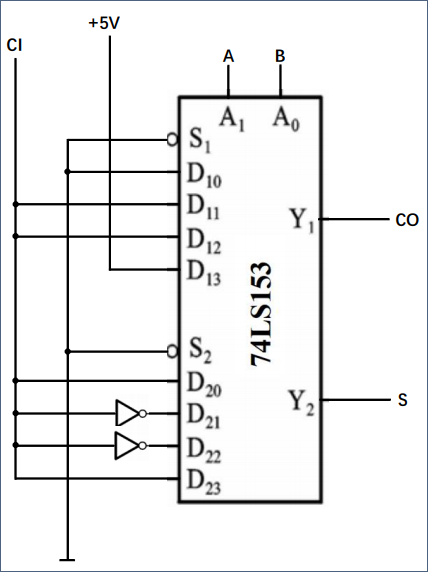
\includegraphics[width=6cm]{Exp04}
   \caption{实验四电路图}
   \label{fig:Exp04}
  \end{figure}

\section{总结}
 \p 本次实验我们使用了多路数据选择器(Multiplexer)。$2^n$ 选 $1$ 多路选择器具有 $n$ 位地址选择位,考虑到输出是由输入决定的,那么至多可以构造出 $(n+1)$ 变量的任意逻辑函数。
 \p 8 选 1 数据选择器 74LS151 有 3 位地址位和 8 位输入。因此可以构造四个变量的任意逻辑函数。
 \p 双 4 选 1 数据选择器 74LS153 有两个相同的 4 选 1 数据选择器。每个数据选择器都有 2 位地址位和 4 位输入,因此可以构造三个变量的任意逻辑函数。2 个数据选择器就可以同时构造任意两个三变量逻辑函数。
 
\section{实验思考题}
\subsection{问题一}
1.试用4选1数据选择器实现一个简单的交通灯故障检测电路。
(要求:每一组信号灯由红、黄、绿三盏灯组成。正常工作情况下,
任何时刻只有一盏灯点亮,而且只允许有一盏灯点亮。而当出现其他五
种点亮状态时,认为电路发生故障,这时要求发出故障信号,以提醒维护人员去修理。)

答:首先指派每个灯的逻辑符号:

红灯亮---A; 黄灯亮---B;绿灯亮---C;

则可以写出逻辑表达式:
\begin{equation}
  Y=ABC+A'BC+AB'C+ABC'+A'B'C'
\end{equation}
即三个灯中有且仅有一盏灯亮时正常,否则发出故障信号。

再指派:
\begin{equation}
  A---A_1;\;B---A_0
\end{equation}
上述逻辑表达式可以写成最小项形式:
\begin{equation}
  Y=m_31+m_1C+m_2C'+m_0C'
\end{equation}
对比数据选择器的输出表达式:$Y=\sum_0^3m_iD_i$。
则可得$D_i$的指派:
\begin{equation}
  D_0---C';D_1---C;D_2---C';D_3---1;
\end{equation}
真值表如表 \ref{tab:T1} 所示。
\begin{table}[H]
  \centering
  \begin{tabular}{|ccc|c|}\hline
   $A$&$B$&$C$ &$Y$
   \\\hline
   0&0&0 &1
   \\\hline
   0&0&1 &0
   \\\hline
   0&1&0 &0
   \\\hline
   0&1&1 &1
   \\\hline
   1&0&0 &0
   \\\hline
   1&0&1 &1
   \\\hline
   1&1&0 &1
   \\\hline
   1&1&1 &1
   \\\hline
  \end{tabular}
  \caption{交通灯检测器真值表}
  \label{tab:T1}
 \end{table}
则由上述分析容易得到电路图如图 \ref{fig:T1} 所示。

\begin{figure}[H]
  \centering
  \fbox{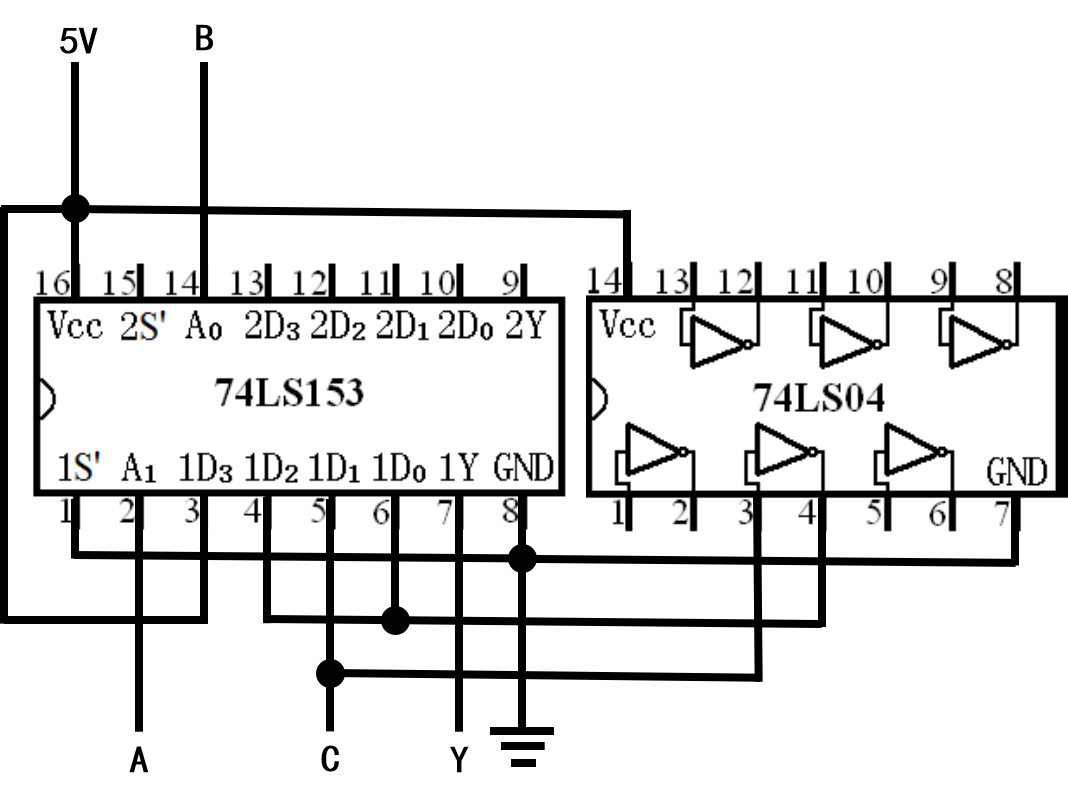
\includegraphics[width=0.6\linewidth]{T1.png}}
  \caption{思考题一电路图}
  \label{fig:T1}
  \end{figure}
\subsection{问题二}
2.数据选择器和译码器都可以实现逻辑函数,试描述他们的特点以及不同之处。

答:译码器将每个二进制代码赋予的特定含义“翻译”过来,转换成相应的信息符号(输出信号)。
其输出特点是将每一个最小项的反输出为其值的反,意即:$Y'_i=m_i'$。

而数据选择器则是根据输入的地址,选择对应地址的信息输出。其输出特点是将每个最小项与其对应的
地址相乘后在求和所有的项,意即:$Y=\sum m_iD_i$。

其最大的不同是数据选择器只有一个输出,而译码器有多个输出端,因此在实现特定逻辑函数时,后者往往需要一个与操作。
而译码器实现逻辑函数非常直接,将逻辑函数表示成多个最小项的非的与/或,然后在输出时将出现的项根据表达式进行与非/或非即可。

而数据选择器有多种实现方式:

一种是存储式实现,将每个最小项对应的值存储在$D_i$中,然后根据输出的最小项表达式将需要的输出值通过或门即可。这种实现方式消耗资源比较大,但是线路和原理很简单。

另一种将逻辑函数表示成最小项的或形式,然后将最后一个逻辑变量$A_n$用$D_i$实现,对比数据选择器的输出函数,将$D_i$指派为$A_n,A_n',0,1$这四种类型,此时$Y$直接对应于输出,
相当于将或门集成在了芯片当中,但需要额外的非门,这个实现较为复杂,但比较节省资源。

\end{document}
